\documentclass{beamer}
\usepackage[utf8]{inputenc}

\usetheme{Madrid}
\usecolortheme{default}
\usepackage{amsmath,amssymb,amsfonts,amsthm}
\usepackage{txfonts}
\usepackage{tkz-euclide}
\usepackage{listings}
\usepackage{adjustbox}
\usepackage{array}
\usepackage{tabularx}
\usepackage{gvv}
\usepackage{lmodern}
\usepackage{circuitikz}
\usepackage{tikz}
\usepackage{graphicx}

\setbeamertemplate{page number in head/foot}[totalframenumber]

\usepackage{tcolorbox}
\tcbuselibrary{minted,breakable,xparse,skins}



\definecolor{bg}{gray}{0.95}
\DeclareTCBListing{mintedbox}{O{}m!O{}}{%
  breakable=true,
  listing engine=minted,
  listing only,
  minted language=#2,
  minted style=default,
  minted options={%
    linenos,
    gobble=0,
    breaklines=true,
    breakafter=,,
    fontsize=\small,
    numbersep=8pt,
    #1},
  boxsep=0pt,
  left skip=0pt,
  right skip=0pt,
  left=25pt,
  right=0pt,
  top=3pt,
  bottom=3pt,
  arc=5pt,
  leftrule=0pt,
  rightrule=0pt,
  bottomrule=2pt,
  toprule=2pt,
  colback=bg,
  colframe=orange!70,
  enhanced,
  overlay={%
    \begin{tcbclipinterior}
    \fill[orange!20!white] (frame.south west) rectangle ([xshift=20pt]frame.north west);
    \end{tcbclipinterior}},
  #3,
}
\lstset{
    language=C,
    basicstyle=\ttfamily\small,
    keywordstyle=\color{blue},
    stringstyle=\color{orange},
    commentstyle=\color{green!60!black},
    numbers=left,
    numberstyle=\tiny\color{gray},
    breaklines=true,
    showstringspaces=false,
}
\title 
{MatGeo Assignment 1.6.22}

\author
{AI25BTECH11007}
\begin{document}

\frame{\titlepage}
\begin{frame}{Question}
Show that the points A(2, -3, 4), B(-1, 2, 1) and C(0, 1/3, 2) are collinear.
\end{frame}
\begin{frame}{Solution}
Let
\begin{equation}
\vec{A}=\myvec{2\\-3\\4},\qquad
\vec{B}=\myvec{-1\\2\\1},\qquad
\vec{C}=\myvec{0\\\tfrac{1}{3}\\2}.
\label{eq:points}
\end{equation}

Form the difference (direction) vectors
\begin{equation}
\overrightarrow{AB}=\vec{B}-\vec{A}=\myvec{-1-2\\[4pt]2-(-3)\\[4pt]1-4}=\myvec{-3\\[4pt]5\\[4pt]-3},
\label{eq:AB}
\end{equation}
\begin{equation}
\overrightarrow{AC}=\vec{C}-\vec{A}=\myvec{0-2\\[4pt]\tfrac{1}{3}-(-3)\\[4pt]2-4}
=\myvec{-2\\[4pt]\tfrac{10}{3}\\[4pt]-2}.
\label{eq:AC}
\end{equation}
\end{frame}
\begin{frame}
Build the $3\times 2$ matrix whose columns are $\overrightarrow{AB}$ and $\overrightarrow{AC}$:
\begin{equation}
\vec{M}=\myvec{\,\overrightarrow{AB}\; & \; \overrightarrow{AC}\,}
=\myvec{ -3 & -2 \\[4pt] 5 & \tfrac{10}{3} \\[4pt] -3 & -2 }.
\label{eq:matrixM}
\end{equation}


We consider the matrix
\begin{equation}
\vec{M} = \myvec{ -3 & -2 \\[4pt] 5 & \tfrac{10}{3} \\[4pt] -3 & -2 }.
\label{eq:M}
\end{equation}

Perform row operations to reduce to echelon form:
\end{frame}
\begin{frame}
    

\[
\begin{aligned}
M &= \myvec{ -3 & -2 \\[4pt] 5 & \tfrac{10}{3} \\[4pt] -3 & -2 } \\[6pt]
&\xrightarrow{R_1 \leftrightarrow R_2}
\myvec{ 5 & \tfrac{10}{3} \\[4pt] -3 & -2 \\[4pt] -3 & -2 } \\[6pt]
&\xrightarrow{R_2 \to 5R_2+3R_1,\;\; R_3 \to 5R_3+3R_1}
\myvec{ 5 & \tfrac{10}{3} \\[4pt] 0 & 0 \\[4pt] 0 & 0 }.
\end{aligned}
\]

Thus, the echelon form of \(M\) has only \(\mathbf{1}\) non-zero row.

\begin{equation}
\operatorname{rank}(M) = 1.
\label{eq:rank}
\end{equation}

Since the rank of the matrix is \(1\), the two direction vectors are linearly dependent, and hence the points \(A,B,C\) are collinear.

\end{frame}
\begin{frame}{Plot}
   \begin{figure}[H]
    \centering
    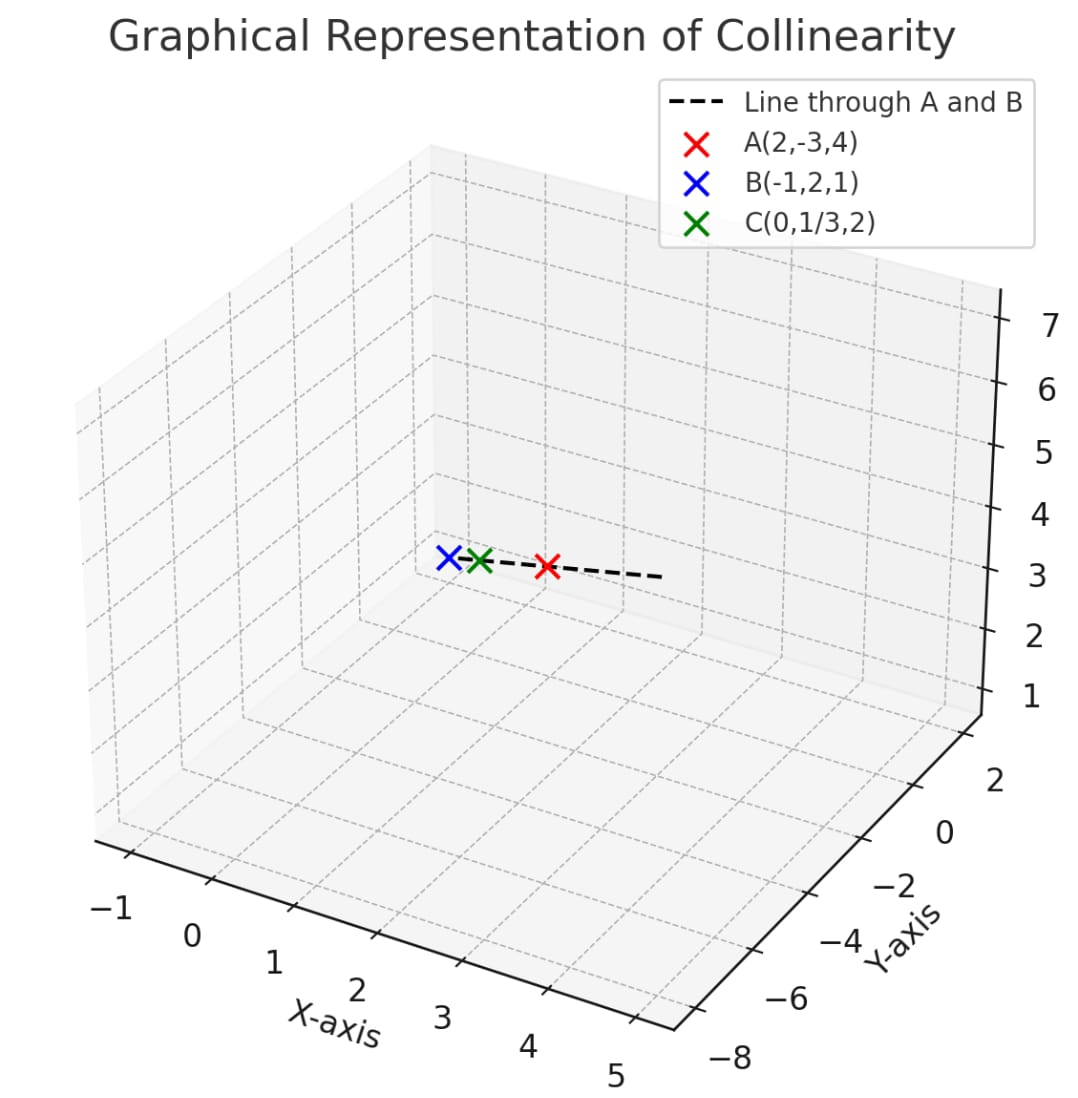
\includegraphics[width=0.6\linewidth]{figs/image.png}
    \caption{Image Visual}
    \label{fig:figs/image.png}
\end{figure}
\end{frame}
\begin{frame}{Conclusion}
    As the rank of the matrix M is 1, the three given points are collinear.
\end{frame}
\end{document}

